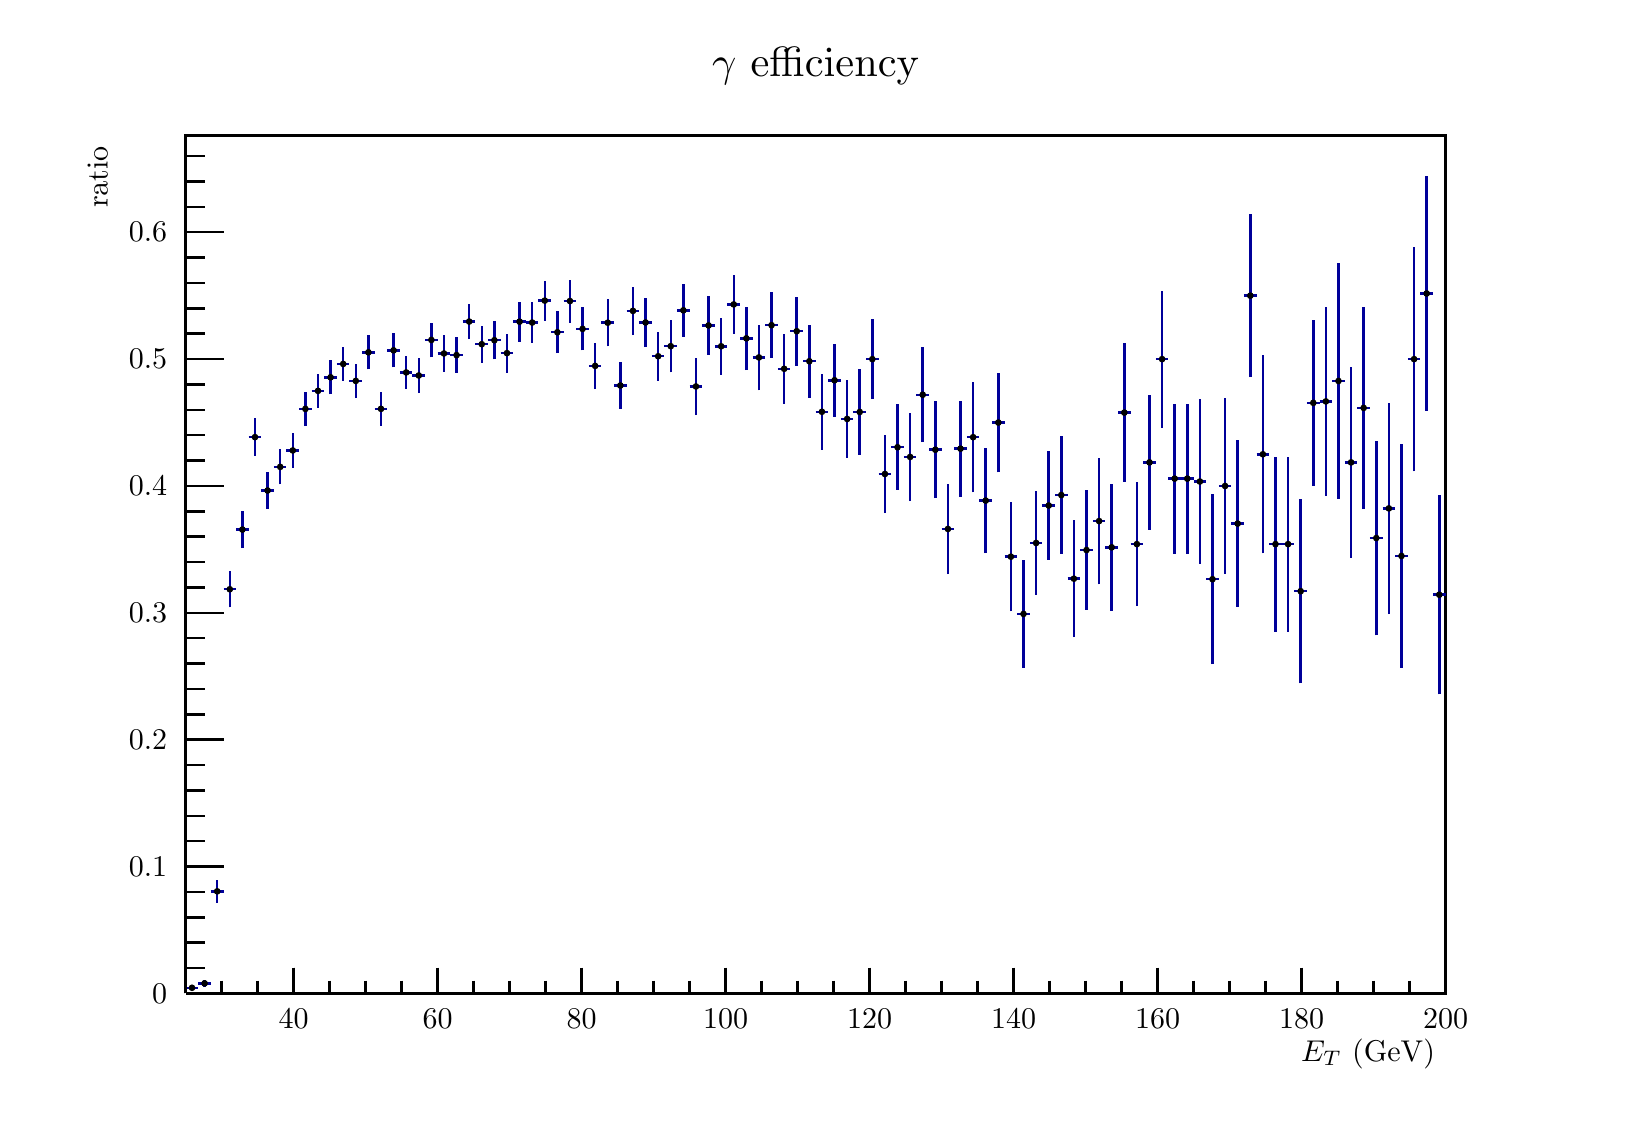
\begin{tikzpicture}
\pgfdeclareplotmark{cross} {
\pgfpathmoveto{\pgfpoint{-0.3\pgfplotmarksize}{\pgfplotmarksize}}
\pgfpathlineto{\pgfpoint{+0.3\pgfplotmarksize}{\pgfplotmarksize}}
\pgfpathlineto{\pgfpoint{+0.3\pgfplotmarksize}{0.3\pgfplotmarksize}}
\pgfpathlineto{\pgfpoint{+1\pgfplotmarksize}{0.3\pgfplotmarksize}}
\pgfpathlineto{\pgfpoint{+1\pgfplotmarksize}{-0.3\pgfplotmarksize}}
\pgfpathlineto{\pgfpoint{+0.3\pgfplotmarksize}{-0.3\pgfplotmarksize}}
\pgfpathlineto{\pgfpoint{+0.3\pgfplotmarksize}{-1.\pgfplotmarksize}}
\pgfpathlineto{\pgfpoint{-0.3\pgfplotmarksize}{-1.\pgfplotmarksize}}
\pgfpathlineto{\pgfpoint{-0.3\pgfplotmarksize}{-0.3\pgfplotmarksize}}
\pgfpathlineto{\pgfpoint{-1.\pgfplotmarksize}{-0.3\pgfplotmarksize}}
\pgfpathlineto{\pgfpoint{-1.\pgfplotmarksize}{0.3\pgfplotmarksize}}
\pgfpathlineto{\pgfpoint{-0.3\pgfplotmarksize}{0.3\pgfplotmarksize}}
\pgfpathclose
\pgfusepathqstroke
}
\pgfdeclareplotmark{cross*} {
\pgfpathmoveto{\pgfpoint{-0.3\pgfplotmarksize}{\pgfplotmarksize}}
\pgfpathlineto{\pgfpoint{+0.3\pgfplotmarksize}{\pgfplotmarksize}}
\pgfpathlineto{\pgfpoint{+0.3\pgfplotmarksize}{0.3\pgfplotmarksize}}
\pgfpathlineto{\pgfpoint{+1\pgfplotmarksize}{0.3\pgfplotmarksize}}
\pgfpathlineto{\pgfpoint{+1\pgfplotmarksize}{-0.3\pgfplotmarksize}}
\pgfpathlineto{\pgfpoint{+0.3\pgfplotmarksize}{-0.3\pgfplotmarksize}}
\pgfpathlineto{\pgfpoint{+0.3\pgfplotmarksize}{-1.\pgfplotmarksize}}
\pgfpathlineto{\pgfpoint{-0.3\pgfplotmarksize}{-1.\pgfplotmarksize}}
\pgfpathlineto{\pgfpoint{-0.3\pgfplotmarksize}{-0.3\pgfplotmarksize}}
\pgfpathlineto{\pgfpoint{-1.\pgfplotmarksize}{-0.3\pgfplotmarksize}}
\pgfpathlineto{\pgfpoint{-1.\pgfplotmarksize}{0.3\pgfplotmarksize}}
\pgfpathlineto{\pgfpoint{-0.3\pgfplotmarksize}{0.3\pgfplotmarksize}}
\pgfpathclose
\pgfusepathqfillstroke
}
\pgfdeclareplotmark{newstar} {
\pgfpathmoveto{\pgfqpoint{0pt}{\pgfplotmarksize}}
\pgfpathlineto{\pgfqpointpolar{44}{0.5\pgfplotmarksize}}
\pgfpathlineto{\pgfqpointpolar{18}{\pgfplotmarksize}}
\pgfpathlineto{\pgfqpointpolar{-20}{0.5\pgfplotmarksize}}
\pgfpathlineto{\pgfqpointpolar{-54}{\pgfplotmarksize}}
\pgfpathlineto{\pgfqpointpolar{-90}{0.5\pgfplotmarksize}}
\pgfpathlineto{\pgfqpointpolar{234}{\pgfplotmarksize}}
\pgfpathlineto{\pgfqpointpolar{198}{0.5\pgfplotmarksize}}
\pgfpathlineto{\pgfqpointpolar{162}{\pgfplotmarksize}}
\pgfpathlineto{\pgfqpointpolar{134}{0.5\pgfplotmarksize}}
\pgfpathclose
\pgfusepathqstroke
}
\pgfdeclareplotmark{newstar*} {
\pgfpathmoveto{\pgfqpoint{0pt}{\pgfplotmarksize}}
\pgfpathlineto{\pgfqpointpolar{44}{0.5\pgfplotmarksize}}
\pgfpathlineto{\pgfqpointpolar{18}{\pgfplotmarksize}}
\pgfpathlineto{\pgfqpointpolar{-20}{0.5\pgfplotmarksize}}
\pgfpathlineto{\pgfqpointpolar{-54}{\pgfplotmarksize}}
\pgfpathlineto{\pgfqpointpolar{-90}{0.5\pgfplotmarksize}}
\pgfpathlineto{\pgfqpointpolar{234}{\pgfplotmarksize}}
\pgfpathlineto{\pgfqpointpolar{198}{0.5\pgfplotmarksize}}
\pgfpathlineto{\pgfqpointpolar{162}{\pgfplotmarksize}}
\pgfpathlineto{\pgfqpointpolar{134}{0.5\pgfplotmarksize}}
\pgfpathclose
\pgfusepathqfillstroke
}
\definecolor{c}{rgb}{1,1,1};
\draw [color=c, fill=c] (0,0) rectangle (20,13.6207);
\draw [color=c, fill=c] (2,1.36207) rectangle (18,12.2586);
\definecolor{c}{rgb}{0,0,0};
\draw [c,line width=0.9] (2,1.36207) -- (2,12.2586) -- (18,12.2586) -- (18,1.36207) -- (2,1.36207);
\definecolor{c}{rgb}{1,1,1};
\draw [color=c, fill=c] (2,1.36207) rectangle (18,12.2586);
\definecolor{c}{rgb}{0,0,0};
\draw [c,line width=0.9] (2,1.36207) -- (2,12.2586) -- (18,12.2586) -- (18,1.36207) -- (2,1.36207);
\definecolor{c}{rgb}{0,0,0.6};
\draw [c,line width=0.9] (2.08,1.39816) -- (2.08,1.43408);
\draw [c,line width=0.9] (2.08,1.43408) -- (2.08,1.47001);
\draw [c,line width=0.9] (2,1.43408) -- (2.08,1.43408);
\draw [c,line width=0.9] (2.08,1.43408) -- (2.16,1.43408);
\definecolor{c}{rgb}{0,0,0};
\foreach \P in {(2.08,1.43408)}{\draw[mark options={color=c,fill=c},mark size=2.402402pt,mark=*,mark size=1pt] plot coordinates {\P};}
\definecolor{c}{rgb}{0,0,0.6};
\draw [c,line width=0.9] (2.24,1.44208) -- (2.24,1.49038);
\draw [c,line width=0.9] (2.24,1.49038) -- (2.24,1.53869);
\draw [c,line width=0.9] (2.16,1.49038) -- (2.24,1.49038);
\draw [c,line width=0.9] (2.24,1.49038) -- (2.32,1.49038);
\definecolor{c}{rgb}{0,0,0};
\foreach \P in {(2.24,1.49038)}{\draw[mark options={color=c,fill=c},mark size=2.402402pt,mark=*,mark size=1pt] plot coordinates {\P};}
\definecolor{c}{rgb}{0,0,0.6};
\draw [c,line width=0.9] (2.4,2.51658) -- (2.4,2.65927);
\draw [c,line width=0.9] (2.4,2.65927) -- (2.4,2.80195);
\draw [c,line width=0.9] (2.32,2.65927) -- (2.4,2.65927);
\draw [c,line width=0.9] (2.4,2.65927) -- (2.48,2.65927);
\definecolor{c}{rgb}{0,0,0};
\foreach \P in {(2.4,2.65927)}{\draw[mark options={color=c,fill=c},mark size=2.402402pt,mark=*,mark size=1pt] plot coordinates {\P};}
\definecolor{c}{rgb}{0,0,0.6};
\draw [c,line width=0.9] (2.56,6.26552) -- (2.56,6.49567);
\draw [c,line width=0.9] (2.56,6.49567) -- (2.56,6.72583);
\draw [c,line width=0.9] (2.48,6.49567) -- (2.56,6.49567);
\draw [c,line width=0.9] (2.56,6.49567) -- (2.64,6.49567);
\definecolor{c}{rgb}{0,0,0};
\foreach \P in {(2.56,6.49567)}{\draw[mark options={color=c,fill=c},mark size=2.402402pt,mark=*,mark size=1pt] plot coordinates {\P};}
\definecolor{c}{rgb}{0,0,0.6};
\draw [c,line width=0.9] (2.72,7.01784) -- (2.72,7.25364);
\draw [c,line width=0.9] (2.72,7.25364) -- (2.72,7.48944);
\draw [c,line width=0.9] (2.64,7.25364) -- (2.72,7.25364);
\draw [c,line width=0.9] (2.72,7.25364) -- (2.8,7.25364);
\definecolor{c}{rgb}{0,0,0};
\foreach \P in {(2.72,7.25364)}{\draw[mark options={color=c,fill=c},mark size=2.402402pt,mark=*,mark size=1pt] plot coordinates {\P};}
\definecolor{c}{rgb}{0,0,0.6};
\draw [c,line width=0.9] (2.88,8.18878) -- (2.88,8.42746);
\draw [c,line width=0.9] (2.88,8.42746) -- (2.88,8.66615);
\draw [c,line width=0.9] (2.8,8.42746) -- (2.88,8.42746);
\draw [c,line width=0.9] (2.88,8.42746) -- (2.96,8.42746);
\definecolor{c}{rgb}{0,0,0};
\foreach \P in {(2.88,8.42746)}{\draw[mark options={color=c,fill=c},mark size=2.402402pt,mark=*,mark size=1pt] plot coordinates {\P};}
\definecolor{c}{rgb}{0,0,0.6};
\draw [c,line width=0.9] (3.04,7.52001) -- (3.04,7.74964);
\draw [c,line width=0.9] (3.04,7.74964) -- (3.04,7.97928);
\draw [c,line width=0.9] (2.96,7.74964) -- (3.04,7.74964);
\draw [c,line width=0.9] (3.04,7.74964) -- (3.12,7.74964);
\definecolor{c}{rgb}{0,0,0};
\foreach \P in {(3.04,7.74964)}{\draw[mark options={color=c,fill=c},mark size=2.402402pt,mark=*,mark size=1pt] plot coordinates {\P};}
\definecolor{c}{rgb}{0,0,0.6};
\draw [c,line width=0.9] (3.2,7.82846) -- (3.2,8.04959);
\draw [c,line width=0.9] (3.2,8.04959) -- (3.2,8.27072);
\draw [c,line width=0.9] (3.12,8.04959) -- (3.2,8.04959);
\draw [c,line width=0.9] (3.2,8.04959) -- (3.28,8.04959);
\definecolor{c}{rgb}{0,0,0};
\foreach \P in {(3.2,8.04959)}{\draw[mark options={color=c,fill=c},mark size=2.402402pt,mark=*,mark size=1pt] plot coordinates {\P};}
\definecolor{c}{rgb}{0,0,0.6};
\draw [c,line width=0.9] (3.36,8.03674) -- (3.36,8.25854);
\draw [c,line width=0.9] (3.36,8.25854) -- (3.36,8.48034);
\draw [c,line width=0.9] (3.28,8.25854) -- (3.36,8.25854);
\draw [c,line width=0.9] (3.36,8.25854) -- (3.44,8.25854);
\definecolor{c}{rgb}{0,0,0};
\foreach \P in {(3.36,8.25854)}{\draw[mark options={color=c,fill=c},mark size=2.402402pt,mark=*,mark size=1pt] plot coordinates {\P};}
\definecolor{c}{rgb}{0,0,0.6};
\draw [c,line width=0.9] (3.52,8.566) -- (3.52,8.78565);
\draw [c,line width=0.9] (3.52,8.78565) -- (3.52,9.0053);
\draw [c,line width=0.9] (3.44,8.78565) -- (3.52,8.78565);
\draw [c,line width=0.9] (3.52,8.78565) -- (3.6,8.78565);
\definecolor{c}{rgb}{0,0,0};
\foreach \P in {(3.52,8.78565)}{\draw[mark options={color=c,fill=c},mark size=2.402402pt,mark=*,mark size=1pt] plot coordinates {\P};}
\definecolor{c}{rgb}{0,0,0.6};
\draw [c,line width=0.9] (3.68,8.80279) -- (3.68,9.01497);
\draw [c,line width=0.9] (3.68,9.01497) -- (3.68,9.22715);
\draw [c,line width=0.9] (3.6,9.01497) -- (3.68,9.01497);
\draw [c,line width=0.9] (3.68,9.01497) -- (3.76,9.01497);
\definecolor{c}{rgb}{0,0,0};
\foreach \P in {(3.68,9.01497)}{\draw[mark options={color=c,fill=c},mark size=2.402402pt,mark=*,mark size=1pt] plot coordinates {\P};}
\definecolor{c}{rgb}{0,0,0.6};
\draw [c,line width=0.9] (3.84,8.97197) -- (3.84,9.1875);
\draw [c,line width=0.9] (3.84,9.1875) -- (3.84,9.40304);
\draw [c,line width=0.9] (3.76,9.1875) -- (3.84,9.1875);
\draw [c,line width=0.9] (3.84,9.1875) -- (3.92,9.1875);
\definecolor{c}{rgb}{0,0,0};
\foreach \P in {(3.84,9.1875)}{\draw[mark options={color=c,fill=c},mark size=2.402402pt,mark=*,mark size=1pt] plot coordinates {\P};}
\definecolor{c}{rgb}{0,0,0.6};
\draw [c,line width=0.9] (4,9.14439) -- (4,9.35676);
\draw [c,line width=0.9] (4,9.35676) -- (4,9.56913);
\draw [c,line width=0.9] (3.92,9.35676) -- (4,9.35676);
\draw [c,line width=0.9] (4,9.35676) -- (4.08,9.35676);
\definecolor{c}{rgb}{0,0,0};
\foreach \P in {(4,9.35676)}{\draw[mark options={color=c,fill=c},mark size=2.402402pt,mark=*,mark size=1pt] plot coordinates {\P};}
\definecolor{c}{rgb}{0,0,0.6};
\draw [c,line width=0.9] (4.16,8.92359) -- (4.16,9.14135);
\draw [c,line width=0.9] (4.16,9.14135) -- (4.16,9.35912);
\draw [c,line width=0.9] (4.08,9.14135) -- (4.16,9.14135);
\draw [c,line width=0.9] (4.16,9.14135) -- (4.24,9.14135);
\definecolor{c}{rgb}{0,0,0};
\foreach \P in {(4.16,9.14135)}{\draw[mark options={color=c,fill=c},mark size=2.402402pt,mark=*,mark size=1pt] plot coordinates {\P};}
\definecolor{c}{rgb}{0,0,0.6};
\draw [c,line width=0.9] (4.32,9.28931) -- (4.32,9.50485);
\draw [c,line width=0.9] (4.32,9.50485) -- (4.32,9.72038);
\draw [c,line width=0.9] (4.24,9.50485) -- (4.32,9.50485);
\draw [c,line width=0.9] (4.32,9.50485) -- (4.4,9.50485);
\definecolor{c}{rgb}{0,0,0};
\foreach \P in {(4.32,9.50485)}{\draw[mark options={color=c,fill=c},mark size=2.402402pt,mark=*,mark size=1pt] plot coordinates {\P};}
\definecolor{c}{rgb}{0,0,0.6};
\draw [c,line width=0.9] (4.48,8.57394) -- (4.48,8.78648);
\draw [c,line width=0.9] (4.48,8.78648) -- (4.48,8.99901);
\draw [c,line width=0.9] (4.4,8.78648) -- (4.48,8.78648);
\draw [c,line width=0.9] (4.48,8.78648) -- (4.56,8.78648);
\definecolor{c}{rgb}{0,0,0};
\foreach \P in {(4.48,8.78648)}{\draw[mark options={color=c,fill=c},mark size=2.402402pt,mark=*,mark size=1pt] plot coordinates {\P};}
\definecolor{c}{rgb}{0,0,0.6};
\draw [c,line width=0.9] (4.64,9.31243) -- (4.64,9.52983);
\draw [c,line width=0.9] (4.64,9.52983) -- (4.64,9.74723);
\draw [c,line width=0.9] (4.56,9.52983) -- (4.64,9.52983);
\draw [c,line width=0.9] (4.64,9.52983) -- (4.72,9.52983);
\definecolor{c}{rgb}{0,0,0};
\foreach \P in {(4.64,9.52983)}{\draw[mark options={color=c,fill=c},mark size=2.402402pt,mark=*,mark size=1pt] plot coordinates {\P};}
\definecolor{c}{rgb}{0,0,0.6};
\draw [c,line width=0.9] (4.8,9.03967) -- (4.8,9.24925);
\draw [c,line width=0.9] (4.8,9.24925) -- (4.8,9.45883);
\draw [c,line width=0.9] (4.72,9.24925) -- (4.8,9.24925);
\draw [c,line width=0.9] (4.8,9.24925) -- (4.88,9.24925);
\definecolor{c}{rgb}{0,0,0};
\foreach \P in {(4.8,9.24925)}{\draw[mark options={color=c,fill=c},mark size=2.402402pt,mark=*,mark size=1pt] plot coordinates {\P};}
\definecolor{c}{rgb}{0,0,0.6};
\draw [c,line width=0.9] (4.96,8.98529) -- (4.96,9.21048);
\draw [c,line width=0.9] (4.96,9.21048) -- (4.96,9.43567);
\draw [c,line width=0.9] (4.88,9.21048) -- (4.96,9.21048);
\draw [c,line width=0.9] (4.96,9.21048) -- (5.04,9.21048);
\definecolor{c}{rgb}{0,0,0};
\foreach \P in {(4.96,9.21048)}{\draw[mark options={color=c,fill=c},mark size=2.402402pt,mark=*,mark size=1pt] plot coordinates {\P};}
\definecolor{c}{rgb}{0,0,0.6};
\draw [c,line width=0.9] (5.12,9.44043) -- (5.12,9.66173);
\draw [c,line width=0.9] (5.12,9.66173) -- (5.12,9.88304);
\draw [c,line width=0.9] (5.04,9.66173) -- (5.12,9.66173);
\draw [c,line width=0.9] (5.12,9.66173) -- (5.2,9.66173);
\definecolor{c}{rgb}{0,0,0};
\foreach \P in {(5.12,9.66173)}{\draw[mark options={color=c,fill=c},mark size=2.402402pt,mark=*,mark size=1pt] plot coordinates {\P};}
\definecolor{c}{rgb}{0,0,0.6};
\draw [c,line width=0.9] (5.28,9.261) -- (5.28,9.48987);
\draw [c,line width=0.9] (5.28,9.48987) -- (5.28,9.71873);
\draw [c,line width=0.9] (5.2,9.48987) -- (5.28,9.48987);
\draw [c,line width=0.9] (5.28,9.48987) -- (5.36,9.48987);
\definecolor{c}{rgb}{0,0,0};
\foreach \P in {(5.28,9.48987)}{\draw[mark options={color=c,fill=c},mark size=2.402402pt,mark=*,mark size=1pt] plot coordinates {\P};}
\definecolor{c}{rgb}{0,0,0.6};
\draw [c,line width=0.9] (5.44,9.24293) -- (5.44,9.46917);
\draw [c,line width=0.9] (5.44,9.46917) -- (5.44,9.69541);
\draw [c,line width=0.9] (5.36,9.46917) -- (5.44,9.46917);
\draw [c,line width=0.9] (5.44,9.46917) -- (5.52,9.46917);
\definecolor{c}{rgb}{0,0,0};
\foreach \P in {(5.44,9.46917)}{\draw[mark options={color=c,fill=c},mark size=2.402402pt,mark=*,mark size=1pt] plot coordinates {\P};}
\definecolor{c}{rgb}{0,0,0.6};
\draw [c,line width=0.9] (5.6,9.67219) -- (5.6,9.89516);
\draw [c,line width=0.9] (5.6,9.89516) -- (5.6,10.1181);
\draw [c,line width=0.9] (5.52,9.89516) -- (5.6,9.89516);
\draw [c,line width=0.9] (5.6,9.89516) -- (5.68,9.89516);
\definecolor{c}{rgb}{0,0,0};
\foreach \P in {(5.6,9.89516)}{\draw[mark options={color=c,fill=c},mark size=2.402402pt,mark=*,mark size=1pt] plot coordinates {\P};}
\definecolor{c}{rgb}{0,0,0.6};
\draw [c,line width=0.9] (5.76,9.37443) -- (5.76,9.6079);
\draw [c,line width=0.9] (5.76,9.6079) -- (5.76,9.84138);
\draw [c,line width=0.9] (5.68,9.6079) -- (5.76,9.6079);
\draw [c,line width=0.9] (5.76,9.6079) -- (5.84,9.6079);
\definecolor{c}{rgb}{0,0,0};
\foreach \P in {(5.76,9.6079)}{\draw[mark options={color=c,fill=c},mark size=2.402402pt,mark=*,mark size=1pt] plot coordinates {\P};}
\definecolor{c}{rgb}{0,0,0.6};
\draw [c,line width=0.9] (5.92,9.41647) -- (5.92,9.6585);
\draw [c,line width=0.9] (5.92,9.6585) -- (5.92,9.90053);
\draw [c,line width=0.9] (5.84,9.6585) -- (5.92,9.6585);
\draw [c,line width=0.9] (5.92,9.6585) -- (6,9.6585);
\definecolor{c}{rgb}{0,0,0};
\foreach \P in {(5.92,9.6585)}{\draw[mark options={color=c,fill=c},mark size=2.402402pt,mark=*,mark size=1pt] plot coordinates {\P};}
\definecolor{c}{rgb}{0,0,0.6};
\draw [c,line width=0.9] (6.08,9.24682) -- (6.08,9.49449);
\draw [c,line width=0.9] (6.08,9.49449) -- (6.08,9.74216);
\draw [c,line width=0.9] (6,9.49449) -- (6.08,9.49449);
\draw [c,line width=0.9] (6.08,9.49449) -- (6.16,9.49449);
\definecolor{c}{rgb}{0,0,0};
\foreach \P in {(6.08,9.49449)}{\draw[mark options={color=c,fill=c},mark size=2.402402pt,mark=*,mark size=1pt] plot coordinates {\P};}
\definecolor{c}{rgb}{0,0,0.6};
\draw [c,line width=0.9] (6.24,9.6418) -- (6.24,9.89411);
\draw [c,line width=0.9] (6.24,9.89411) -- (6.24,10.1464);
\draw [c,line width=0.9] (6.16,9.89411) -- (6.24,9.89411);
\draw [c,line width=0.9] (6.24,9.89411) -- (6.32,9.89411);
\definecolor{c}{rgb}{0,0,0};
\foreach \P in {(6.24,9.89411)}{\draw[mark options={color=c,fill=c},mark size=2.402402pt,mark=*,mark size=1pt] plot coordinates {\P};}
\definecolor{c}{rgb}{0,0,0.6};
\draw [c,line width=0.9] (6.4,9.62691) -- (6.4,9.88266);
\draw [c,line width=0.9] (6.4,9.88266) -- (6.4,10.1384);
\draw [c,line width=0.9] (6.32,9.88266) -- (6.4,9.88266);
\draw [c,line width=0.9] (6.4,9.88266) -- (6.48,9.88266);
\definecolor{c}{rgb}{0,0,0};
\foreach \P in {(6.4,9.88266)}{\draw[mark options={color=c,fill=c},mark size=2.402402pt,mark=*,mark size=1pt] plot coordinates {\P};}
\definecolor{c}{rgb}{0,0,0.6};
\draw [c,line width=0.9] (6.56,9.90578) -- (6.56,10.1611);
\draw [c,line width=0.9] (6.56,10.1611) -- (6.56,10.4165);
\draw [c,line width=0.9] (6.48,10.1611) -- (6.56,10.1611);
\draw [c,line width=0.9] (6.56,10.1611) -- (6.64,10.1611);
\definecolor{c}{rgb}{0,0,0};
\foreach \P in {(6.56,10.1611)}{\draw[mark options={color=c,fill=c},mark size=2.402402pt,mark=*,mark size=1pt] plot coordinates {\P};}
\definecolor{c}{rgb}{0,0,0.6};
\draw [c,line width=0.9] (6.72,9.49426) -- (6.72,9.75949);
\draw [c,line width=0.9] (6.72,9.75949) -- (6.72,10.0247);
\draw [c,line width=0.9] (6.64,9.75949) -- (6.72,9.75949);
\draw [c,line width=0.9] (6.72,9.75949) -- (6.8,9.75949);
\definecolor{c}{rgb}{0,0,0};
\foreach \P in {(6.72,9.75949)}{\draw[mark options={color=c,fill=c},mark size=2.402402pt,mark=*,mark size=1pt] plot coordinates {\P};}
\definecolor{c}{rgb}{0,0,0.6};
\draw [c,line width=0.9] (6.88,9.88274) -- (6.88,10.1558);
\draw [c,line width=0.9] (6.88,10.1558) -- (6.88,10.4289);
\draw [c,line width=0.9] (6.8,10.1558) -- (6.88,10.1558);
\draw [c,line width=0.9] (6.88,10.1558) -- (6.96,10.1558);
\definecolor{c}{rgb}{0,0,0};
\foreach \P in {(6.88,10.1558)}{\draw[mark options={color=c,fill=c},mark size=2.402402pt,mark=*,mark size=1pt] plot coordinates {\P};}
\definecolor{c}{rgb}{0,0,0.6};
\draw [c,line width=0.9] (7.04,9.52773) -- (7.04,9.80198);
\draw [c,line width=0.9] (7.04,9.80198) -- (7.04,10.0762);
\draw [c,line width=0.9] (6.96,9.80198) -- (7.04,9.80198);
\draw [c,line width=0.9] (7.04,9.80198) -- (7.12,9.80198);
\definecolor{c}{rgb}{0,0,0};
\foreach \P in {(7.04,9.80198)}{\draw[mark options={color=c,fill=c},mark size=2.402402pt,mark=*,mark size=1pt] plot coordinates {\P};}
\definecolor{c}{rgb}{0,0,0.6};
\draw [c,line width=0.9] (7.2,9.037) -- (7.2,9.33195);
\draw [c,line width=0.9] (7.2,9.33195) -- (7.2,9.62689);
\draw [c,line width=0.9] (7.12,9.33195) -- (7.2,9.33195);
\draw [c,line width=0.9] (7.2,9.33195) -- (7.28,9.33195);
\definecolor{c}{rgb}{0,0,0};
\foreach \P in {(7.2,9.33195)}{\draw[mark options={color=c,fill=c},mark size=2.402402pt,mark=*,mark size=1pt] plot coordinates {\P};}
\definecolor{c}{rgb}{0,0,0.6};
\draw [c,line width=0.9] (7.36,9.57952) -- (7.36,9.88031);
\draw [c,line width=0.9] (7.36,9.88031) -- (7.36,10.1811);
\draw [c,line width=0.9] (7.28,9.88031) -- (7.36,9.88031);
\draw [c,line width=0.9] (7.36,9.88031) -- (7.44,9.88031);
\definecolor{c}{rgb}{0,0,0};
\foreach \P in {(7.36,9.88031)}{\draw[mark options={color=c,fill=c},mark size=2.402402pt,mark=*,mark size=1pt] plot coordinates {\P};}
\definecolor{c}{rgb}{0,0,0.6};
\draw [c,line width=0.9] (7.52,8.78821) -- (7.52,9.08312);
\draw [c,line width=0.9] (7.52,9.08312) -- (7.52,9.37802);
\draw [c,line width=0.9] (7.44,9.08312) -- (7.52,9.08312);
\draw [c,line width=0.9] (7.52,9.08312) -- (7.6,9.08312);
\definecolor{c}{rgb}{0,0,0};
\foreach \P in {(7.52,9.08312)}{\draw[mark options={color=c,fill=c},mark size=2.402402pt,mark=*,mark size=1pt] plot coordinates {\P};}
\definecolor{c}{rgb}{0,0,0.6};
\draw [c,line width=0.9] (7.68,9.72366) -- (7.68,10.0308);
\draw [c,line width=0.9] (7.68,10.0308) -- (7.68,10.338);
\draw [c,line width=0.9] (7.6,10.0308) -- (7.68,10.0308);
\draw [c,line width=0.9] (7.68,10.0308) -- (7.76,10.0308);
\definecolor{c}{rgb}{0,0,0};
\foreach \P in {(7.68,10.0308)}{\draw[mark options={color=c,fill=c},mark size=2.402402pt,mark=*,mark size=1pt] plot coordinates {\P};}
\definecolor{c}{rgb}{0,0,0.6};
\draw [c,line width=0.9] (7.84,9.57006) -- (7.84,9.8836);
\draw [c,line width=0.9] (7.84,9.8836) -- (7.84,10.1971);
\draw [c,line width=0.9] (7.76,9.8836) -- (7.84,9.8836);
\draw [c,line width=0.9] (7.84,9.8836) -- (7.92,9.8836);
\definecolor{c}{rgb}{0,0,0};
\foreach \P in {(7.84,9.8836)}{\draw[mark options={color=c,fill=c},mark size=2.402402pt,mark=*,mark size=1pt] plot coordinates {\P};}
\definecolor{c}{rgb}{0,0,0.6};
\draw [c,line width=0.9] (8,9.14119) -- (8,9.45502);
\draw [c,line width=0.9] (8,9.45502) -- (8,9.76884);
\draw [c,line width=0.9] (7.92,9.45502) -- (8,9.45502);
\draw [c,line width=0.9] (8,9.45502) -- (8.08,9.45502);
\definecolor{c}{rgb}{0,0,0};
\foreach \P in {(8,9.45502)}{\draw[mark options={color=c,fill=c},mark size=2.402402pt,mark=*,mark size=1pt] plot coordinates {\P};}
\definecolor{c}{rgb}{0,0,0.6};
\draw [c,line width=0.9] (8.16,9.25059) -- (8.16,9.58276);
\draw [c,line width=0.9] (8.16,9.58276) -- (8.16,9.91492);
\draw [c,line width=0.9] (8.08,9.58276) -- (8.16,9.58276);
\draw [c,line width=0.9] (8.16,9.58276) -- (8.24,9.58276);
\definecolor{c}{rgb}{0,0,0};
\foreach \P in {(8.16,9.58276)}{\draw[mark options={color=c,fill=c},mark size=2.402402pt,mark=*,mark size=1pt] plot coordinates {\P};}
\definecolor{c}{rgb}{0,0,0.6};
\draw [c,line width=0.9] (8.32,9.70221) -- (8.32,10.0381);
\draw [c,line width=0.9] (8.32,10.0381) -- (8.32,10.3739);
\draw [c,line width=0.9] (8.24,10.0381) -- (8.32,10.0381);
\draw [c,line width=0.9] (8.32,10.0381) -- (8.4,10.0381);
\definecolor{c}{rgb}{0,0,0};
\foreach \P in {(8.32,10.0381)}{\draw[mark options={color=c,fill=c},mark size=2.402402pt,mark=*,mark size=1pt] plot coordinates {\P};}
\definecolor{c}{rgb}{0,0,0.6};
\draw [c,line width=0.9] (8.48,8.70622) -- (8.48,9.07095);
\draw [c,line width=0.9] (8.48,9.07095) -- (8.48,9.43567);
\draw [c,line width=0.9] (8.4,9.07095) -- (8.48,9.07095);
\draw [c,line width=0.9] (8.48,9.07095) -- (8.56,9.07095);
\definecolor{c}{rgb}{0,0,0};
\foreach \P in {(8.48,9.07095)}{\draw[mark options={color=c,fill=c},mark size=2.402402pt,mark=*,mark size=1pt] plot coordinates {\P};}
\definecolor{c}{rgb}{0,0,0.6};
\draw [c,line width=0.9] (8.64,9.47527) -- (8.64,9.84596);
\draw [c,line width=0.9] (8.64,9.84596) -- (8.64,10.2166);
\draw [c,line width=0.9] (8.56,9.84596) -- (8.64,9.84596);
\draw [c,line width=0.9] (8.64,9.84596) -- (8.72,9.84596);
\definecolor{c}{rgb}{0,0,0};
\foreach \P in {(8.64,9.84596)}{\draw[mark options={color=c,fill=c},mark size=2.402402pt,mark=*,mark size=1pt] plot coordinates {\P};}
\definecolor{c}{rgb}{0,0,0.6};
\draw [c,line width=0.9] (8.8,9.21903) -- (8.8,9.58143);
\draw [c,line width=0.9] (8.8,9.58143) -- (8.8,9.94382);
\draw [c,line width=0.9] (8.72,9.58143) -- (8.8,9.58143);
\draw [c,line width=0.9] (8.8,9.58143) -- (8.88,9.58143);
\definecolor{c}{rgb}{0,0,0};
\foreach \P in {(8.8,9.58143)}{\draw[mark options={color=c,fill=c},mark size=2.402402pt,mark=*,mark size=1pt] plot coordinates {\P};}
\definecolor{c}{rgb}{0,0,0.6};
\draw [c,line width=0.9] (8.96,9.74024) -- (8.96,10.1128);
\draw [c,line width=0.9] (8.96,10.1128) -- (8.96,10.4855);
\draw [c,line width=0.9] (8.88,10.1128) -- (8.96,10.1128);
\draw [c,line width=0.9] (8.96,10.1128) -- (9.04,10.1128);
\definecolor{c}{rgb}{0,0,0};
\foreach \P in {(8.96,10.1128)}{\draw[mark options={color=c,fill=c},mark size=2.402402pt,mark=*,mark size=1pt] plot coordinates {\P};}
\definecolor{c}{rgb}{0,0,0.6};
\draw [c,line width=0.9] (9.12,9.27803) -- (9.12,9.68215);
\draw [c,line width=0.9] (9.12,9.68215) -- (9.12,10.0863);
\draw [c,line width=0.9] (9.04,9.68215) -- (9.12,9.68215);
\draw [c,line width=0.9] (9.12,9.68215) -- (9.2,9.68215);
\definecolor{c}{rgb}{0,0,0};
\foreach \P in {(9.12,9.68215)}{\draw[mark options={color=c,fill=c},mark size=2.402402pt,mark=*,mark size=1pt] plot coordinates {\P};}
\definecolor{c}{rgb}{0,0,0.6};
\draw [c,line width=0.9] (9.28,9.02281) -- (9.28,9.43994);
\draw [c,line width=0.9] (9.28,9.43994) -- (9.28,9.85708);
\draw [c,line width=0.9] (9.2,9.43994) -- (9.28,9.43994);
\draw [c,line width=0.9] (9.28,9.43994) -- (9.36,9.43994);
\definecolor{c}{rgb}{0,0,0};
\foreach \P in {(9.28,9.43994)}{\draw[mark options={color=c,fill=c},mark size=2.402402pt,mark=*,mark size=1pt] plot coordinates {\P};}
\definecolor{c}{rgb}{0,0,0.6};
\draw [c,line width=0.9] (9.44,9.43318) -- (9.44,9.84916);
\draw [c,line width=0.9] (9.44,9.84916) -- (9.44,10.2651);
\draw [c,line width=0.9] (9.36,9.84916) -- (9.44,9.84916);
\draw [c,line width=0.9] (9.44,9.84916) -- (9.52,9.84916);
\definecolor{c}{rgb}{0,0,0};
\foreach \P in {(9.44,9.84916)}{\draw[mark options={color=c,fill=c},mark size=2.402402pt,mark=*,mark size=1pt] plot coordinates {\P};}
\definecolor{c}{rgb}{0,0,0.6};
\draw [c,line width=0.9] (9.6,8.8497) -- (9.6,9.29516);
\draw [c,line width=0.9] (9.6,9.29516) -- (9.6,9.74062);
\draw [c,line width=0.9] (9.52,9.29516) -- (9.6,9.29516);
\draw [c,line width=0.9] (9.6,9.29516) -- (9.68,9.29516);
\definecolor{c}{rgb}{0,0,0};
\foreach \P in {(9.6,9.29516)}{\draw[mark options={color=c,fill=c},mark size=2.402402pt,mark=*,mark size=1pt] plot coordinates {\P};}
\definecolor{c}{rgb}{0,0,0.6};
\draw [c,line width=0.9] (9.76,9.33687) -- (9.76,9.77272);
\draw [c,line width=0.9] (9.76,9.77272) -- (9.76,10.2086);
\draw [c,line width=0.9] (9.68,9.77272) -- (9.76,9.77272);
\draw [c,line width=0.9] (9.76,9.77272) -- (9.84,9.77272);
\definecolor{c}{rgb}{0,0,0};
\foreach \P in {(9.76,9.77272)}{\draw[mark options={color=c,fill=c},mark size=2.402402pt,mark=*,mark size=1pt] plot coordinates {\P};}
\definecolor{c}{rgb}{0,0,0.6};
\draw [c,line width=0.9] (9.92,8.9255) -- (9.92,9.3914);
\draw [c,line width=0.9] (9.92,9.3914) -- (9.92,9.8573);
\draw [c,line width=0.9] (9.84,9.3914) -- (9.92,9.3914);
\draw [c,line width=0.9] (9.92,9.3914) -- (10,9.3914);
\definecolor{c}{rgb}{0,0,0};
\foreach \P in {(9.92,9.3914)}{\draw[mark options={color=c,fill=c},mark size=2.402402pt,mark=*,mark size=1pt] plot coordinates {\P};}
\definecolor{c}{rgb}{0,0,0.6};
\draw [c,line width=0.9] (10.08,8.26703) -- (10.08,8.74941);
\draw [c,line width=0.9] (10.08,8.74941) -- (10.08,9.23179);
\draw [c,line width=0.9] (10,8.74941) -- (10.08,8.74941);
\draw [c,line width=0.9] (10.08,8.74941) -- (10.16,8.74941);
\definecolor{c}{rgb}{0,0,0};
\foreach \P in {(10.08,8.74941)}{\draw[mark options={color=c,fill=c},mark size=2.402402pt,mark=*,mark size=1pt] plot coordinates {\P};}
\definecolor{c}{rgb}{0,0,0.6};
\draw [c,line width=0.9] (10.24,8.68493) -- (10.24,9.1498);
\draw [c,line width=0.9] (10.24,9.1498) -- (10.24,9.61467);
\draw [c,line width=0.9] (10.16,9.1498) -- (10.24,9.1498);
\draw [c,line width=0.9] (10.24,9.1498) -- (10.32,9.1498);
\definecolor{c}{rgb}{0,0,0};
\foreach \P in {(10.24,9.1498)}{\draw[mark options={color=c,fill=c},mark size=2.402402pt,mark=*,mark size=1pt] plot coordinates {\P};}
\definecolor{c}{rgb}{0,0,0.6};
\draw [c,line width=0.9] (10.4,8.16563) -- (10.4,8.65832);
\draw [c,line width=0.9] (10.4,8.65832) -- (10.4,9.151);
\draw [c,line width=0.9] (10.32,8.65832) -- (10.4,8.65832);
\draw [c,line width=0.9] (10.4,8.65832) -- (10.48,8.65832);
\definecolor{c}{rgb}{0,0,0};
\foreach \P in {(10.4,8.65832)}{\draw[mark options={color=c,fill=c},mark size=2.402402pt,mark=*,mark size=1pt] plot coordinates {\P};}
\definecolor{c}{rgb}{0,0,0.6};
\draw [c,line width=0.9] (10.56,8.20073) -- (10.56,8.74699);
\draw [c,line width=0.9] (10.56,8.74699) -- (10.56,9.29324);
\draw [c,line width=0.9] (10.48,8.74699) -- (10.56,8.74699);
\draw [c,line width=0.9] (10.56,8.74699) -- (10.64,8.74699);
\definecolor{c}{rgb}{0,0,0};
\foreach \P in {(10.56,8.74699)}{\draw[mark options={color=c,fill=c},mark size=2.402402pt,mark=*,mark size=1pt] plot coordinates {\P};}
\definecolor{c}{rgb}{0,0,0.6};
\draw [c,line width=0.9] (10.72,8.90882) -- (10.72,9.41834);
\draw [c,line width=0.9] (10.72,9.41834) -- (10.72,9.92787);
\draw [c,line width=0.9] (10.64,9.41834) -- (10.72,9.41834);
\draw [c,line width=0.9] (10.72,9.41834) -- (10.8,9.41834);
\definecolor{c}{rgb}{0,0,0};
\foreach \P in {(10.72,9.41834)}{\draw[mark options={color=c,fill=c},mark size=2.402402pt,mark=*,mark size=1pt] plot coordinates {\P};}
\definecolor{c}{rgb}{0,0,0.6};
\draw [c,line width=0.9] (10.88,7.4622) -- (10.88,7.95933);
\draw [c,line width=0.9] (10.88,7.95933) -- (10.88,8.45647);
\draw [c,line width=0.9] (10.8,7.95933) -- (10.88,7.95933);
\draw [c,line width=0.9] (10.88,7.95933) -- (10.96,7.95933);
\definecolor{c}{rgb}{0,0,0};
\foreach \P in {(10.88,7.95933)}{\draw[mark options={color=c,fill=c},mark size=2.402402pt,mark=*,mark size=1pt] plot coordinates {\P};}
\definecolor{c}{rgb}{0,0,0.6};
\draw [c,line width=0.9] (11.04,7.75657) -- (11.04,8.29942);
\draw [c,line width=0.9] (11.04,8.29942) -- (11.04,8.84226);
\draw [c,line width=0.9] (10.96,8.29942) -- (11.04,8.29942);
\draw [c,line width=0.9] (11.04,8.29942) -- (11.12,8.29942);
\definecolor{c}{rgb}{0,0,0};
\foreach \P in {(11.04,8.29942)}{\draw[mark options={color=c,fill=c},mark size=2.402402pt,mark=*,mark size=1pt] plot coordinates {\P};}
\definecolor{c}{rgb}{0,0,0.6};
\draw [c,line width=0.9] (11.2,7.61439) -- (11.2,8.17583);
\draw [c,line width=0.9] (11.2,8.17583) -- (11.2,8.73728);
\draw [c,line width=0.9] (11.12,8.17583) -- (11.2,8.17583);
\draw [c,line width=0.9] (11.2,8.17583) -- (11.28,8.17583);
\definecolor{c}{rgb}{0,0,0};
\foreach \P in {(11.2,8.17583)}{\draw[mark options={color=c,fill=c},mark size=2.402402pt,mark=*,mark size=1pt] plot coordinates {\P};}
\definecolor{c}{rgb}{0,0,0.6};
\draw [c,line width=0.9] (11.36,8.36285) -- (11.36,8.96574);
\draw [c,line width=0.9] (11.36,8.96574) -- (11.36,9.56863);
\draw [c,line width=0.9] (11.28,8.96574) -- (11.36,8.96574);
\draw [c,line width=0.9] (11.36,8.96574) -- (11.44,8.96574);
\definecolor{c}{rgb}{0,0,0};
\foreach \P in {(11.36,8.96574)}{\draw[mark options={color=c,fill=c},mark size=2.402402pt,mark=*,mark size=1pt] plot coordinates {\P};}
\definecolor{c}{rgb}{0,0,0.6};
\draw [c,line width=0.9] (11.52,7.65227) -- (11.52,8.26745);
\draw [c,line width=0.9] (11.52,8.26745) -- (11.52,8.88263);
\draw [c,line width=0.9] (11.44,8.26745) -- (11.52,8.26745);
\draw [c,line width=0.9] (11.52,8.26745) -- (11.6,8.26745);
\definecolor{c}{rgb}{0,0,0};
\foreach \P in {(11.52,8.26745)}{\draw[mark options={color=c,fill=c},mark size=2.402402pt,mark=*,mark size=1pt] plot coordinates {\P};}
\definecolor{c}{rgb}{0,0,0.6};
\draw [c,line width=0.9] (11.68,6.68741) -- (11.68,7.2612);
\draw [c,line width=0.9] (11.68,7.2612) -- (11.68,7.83499);
\draw [c,line width=0.9] (11.6,7.2612) -- (11.68,7.2612);
\draw [c,line width=0.9] (11.68,7.2612) -- (11.76,7.2612);
\definecolor{c}{rgb}{0,0,0};
\foreach \P in {(11.68,7.2612)}{\draw[mark options={color=c,fill=c},mark size=2.402402pt,mark=*,mark size=1pt] plot coordinates {\P};}
\definecolor{c}{rgb}{0,0,0.6};
\draw [c,line width=0.9] (11.84,7.66929) -- (11.84,8.28099);
\draw [c,line width=0.9] (11.84,8.28099) -- (11.84,8.89269);
\draw [c,line width=0.9] (11.76,8.28099) -- (11.84,8.28099);
\draw [c,line width=0.9] (11.84,8.28099) -- (11.92,8.28099);
\definecolor{c}{rgb}{0,0,0};
\foreach \P in {(11.84,8.28099)}{\draw[mark options={color=c,fill=c},mark size=2.402402pt,mark=*,mark size=1pt] plot coordinates {\P};}
\definecolor{c}{rgb}{0,0,0.6};
\draw [c,line width=0.9] (12,7.72559) -- (12,8.4268);
\draw [c,line width=0.9] (12,8.4268) -- (12,9.12801);
\draw [c,line width=0.9] (11.92,8.4268) -- (12,8.4268);
\draw [c,line width=0.9] (12,8.4268) -- (12.08,8.4268);
\definecolor{c}{rgb}{0,0,0};
\foreach \P in {(12,8.4268)}{\draw[mark options={color=c,fill=c},mark size=2.402402pt,mark=*,mark size=1pt] plot coordinates {\P};}
\definecolor{c}{rgb}{0,0,0.6};
\draw [c,line width=0.9] (12.16,6.95551) -- (12.16,7.62162);
\draw [c,line width=0.9] (12.16,7.62162) -- (12.16,8.28773);
\draw [c,line width=0.9] (12.08,7.62162) -- (12.16,7.62162);
\draw [c,line width=0.9] (12.16,7.62162) -- (12.24,7.62162);
\definecolor{c}{rgb}{0,0,0};
\foreach \P in {(12.16,7.62162)}{\draw[mark options={color=c,fill=c},mark size=2.402402pt,mark=*,mark size=1pt] plot coordinates {\P};}
\definecolor{c}{rgb}{0,0,0.6};
\draw [c,line width=0.9] (12.32,7.979) -- (12.32,8.61272);
\draw [c,line width=0.9] (12.32,8.61272) -- (12.32,9.24643);
\draw [c,line width=0.9] (12.24,8.61272) -- (12.32,8.61272);
\draw [c,line width=0.9] (12.32,8.61272) -- (12.4,8.61272);
\definecolor{c}{rgb}{0,0,0};
\foreach \P in {(12.32,8.61272)}{\draw[mark options={color=c,fill=c},mark size=2.402402pt,mark=*,mark size=1pt] plot coordinates {\P};}
\definecolor{c}{rgb}{0,0,0.6};
\draw [c,line width=0.9] (12.48,6.21591) -- (12.48,6.90901);
\draw [c,line width=0.9] (12.48,6.90901) -- (12.48,7.60211);
\draw [c,line width=0.9] (12.4,6.90901) -- (12.48,6.90901);
\draw [c,line width=0.9] (12.48,6.90901) -- (12.56,6.90901);
\definecolor{c}{rgb}{0,0,0};
\foreach \P in {(12.48,6.90901)}{\draw[mark options={color=c,fill=c},mark size=2.402402pt,mark=*,mark size=1pt] plot coordinates {\P};}
\definecolor{c}{rgb}{0,0,0.6};
\draw [c,line width=0.9] (12.64,5.5) -- (12.64,6.18206);
\draw [c,line width=0.9] (12.64,6.18206) -- (12.64,6.86413);
\draw [c,line width=0.9] (12.56,6.18206) -- (12.64,6.18206);
\draw [c,line width=0.9] (12.64,6.18206) -- (12.72,6.18206);
\definecolor{c}{rgb}{0,0,0};
\foreach \P in {(12.64,6.18206)}{\draw[mark options={color=c,fill=c},mark size=2.402402pt,mark=*,mark size=1pt] plot coordinates {\P};}
\definecolor{c}{rgb}{0,0,0.6};
\draw [c,line width=0.9] (12.8,6.42684) -- (12.8,7.08319);
\draw [c,line width=0.9] (12.8,7.08319) -- (12.8,7.73955);
\draw [c,line width=0.9] (12.72,7.08319) -- (12.8,7.08319);
\draw [c,line width=0.9] (12.8,7.08319) -- (12.88,7.08319);
\definecolor{c}{rgb}{0,0,0};
\foreach \P in {(12.8,7.08319)}{\draw[mark options={color=c,fill=c},mark size=2.402402pt,mark=*,mark size=1pt] plot coordinates {\P};}
\definecolor{c}{rgb}{0,0,0.6};
\draw [c,line width=0.9] (12.96,6.87169) -- (12.96,7.5592);
\draw [c,line width=0.9] (12.96,7.5592) -- (12.96,8.24671);
\draw [c,line width=0.9] (12.88,7.5592) -- (12.96,7.5592);
\draw [c,line width=0.9] (12.96,7.5592) -- (13.04,7.5592);
\definecolor{c}{rgb}{0,0,0};
\foreach \P in {(12.96,7.5592)}{\draw[mark options={color=c,fill=c},mark size=2.402402pt,mark=*,mark size=1pt] plot coordinates {\P};}
\definecolor{c}{rgb}{0,0,0.6};
\draw [c,line width=0.9] (13.12,6.94844) -- (13.12,7.692);
\draw [c,line width=0.9] (13.12,7.692) -- (13.12,8.43556);
\draw [c,line width=0.9] (13.04,7.692) -- (13.12,7.692);
\draw [c,line width=0.9] (13.12,7.692) -- (13.2,7.692);
\definecolor{c}{rgb}{0,0,0};
\foreach \P in {(13.12,7.692)}{\draw[mark options={color=c,fill=c},mark size=2.402402pt,mark=*,mark size=1pt] plot coordinates {\P};}
\definecolor{c}{rgb}{0,0,0.6};
\draw [c,line width=0.9] (13.28,5.88849) -- (13.28,6.62963);
\draw [c,line width=0.9] (13.28,6.62963) -- (13.28,7.37078);
\draw [c,line width=0.9] (13.2,6.62963) -- (13.28,6.62963);
\draw [c,line width=0.9] (13.28,6.62963) -- (13.36,6.62963);
\definecolor{c}{rgb}{0,0,0};
\foreach \P in {(13.28,6.62963)}{\draw[mark options={color=c,fill=c},mark size=2.402402pt,mark=*,mark size=1pt] plot coordinates {\P};}
\definecolor{c}{rgb}{0,0,0.6};
\draw [c,line width=0.9] (13.44,6.23664) -- (13.44,6.99364);
\draw [c,line width=0.9] (13.44,6.99364) -- (13.44,7.75064);
\draw [c,line width=0.9] (13.36,6.99364) -- (13.44,6.99364);
\draw [c,line width=0.9] (13.44,6.99364) -- (13.52,6.99364);
\definecolor{c}{rgb}{0,0,0};
\foreach \P in {(13.44,6.99364)}{\draw[mark options={color=c,fill=c},mark size=2.402402pt,mark=*,mark size=1pt] plot coordinates {\P};}
\definecolor{c}{rgb}{0,0,0.6};
\draw [c,line width=0.9] (13.6,6.55802) -- (13.6,7.36142);
\draw [c,line width=0.9] (13.6,7.36142) -- (13.6,8.16482);
\draw [c,line width=0.9] (13.52,7.36142) -- (13.6,7.36142);
\draw [c,line width=0.9] (13.6,7.36142) -- (13.68,7.36142);
\definecolor{c}{rgb}{0,0,0};
\foreach \P in {(13.6,7.36142)}{\draw[mark options={color=c,fill=c},mark size=2.402402pt,mark=*,mark size=1pt] plot coordinates {\P};}
\definecolor{c}{rgb}{0,0,0.6};
\draw [c,line width=0.9] (13.76,6.22152) -- (13.76,7.02802);
\draw [c,line width=0.9] (13.76,7.02802) -- (13.76,7.83452);
\draw [c,line width=0.9] (13.68,7.02802) -- (13.76,7.02802);
\draw [c,line width=0.9] (13.76,7.02802) -- (13.84,7.02802);
\definecolor{c}{rgb}{0,0,0};
\foreach \P in {(13.76,7.02802)}{\draw[mark options={color=c,fill=c},mark size=2.402402pt,mark=*,mark size=1pt] plot coordinates {\P};}
\definecolor{c}{rgb}{0,0,0.6};
\draw [c,line width=0.9] (13.92,7.85776) -- (13.92,8.7389);
\draw [c,line width=0.9] (13.92,8.7389) -- (13.92,9.62004);
\draw [c,line width=0.9] (13.84,8.7389) -- (13.92,8.7389);
\draw [c,line width=0.9] (13.92,8.7389) -- (14,8.7389);
\definecolor{c}{rgb}{0,0,0};
\foreach \P in {(13.92,8.7389)}{\draw[mark options={color=c,fill=c},mark size=2.402402pt,mark=*,mark size=1pt] plot coordinates {\P};}
\definecolor{c}{rgb}{0,0,0.6};
\draw [c,line width=0.9] (14.08,6.28211) -- (14.08,7.0686);
\draw [c,line width=0.9] (14.08,7.0686) -- (14.08,7.85509);
\draw [c,line width=0.9] (14,7.0686) -- (14.08,7.0686);
\draw [c,line width=0.9] (14.08,7.0686) -- (14.16,7.0686);
\definecolor{c}{rgb}{0,0,0};
\foreach \P in {(14.08,7.0686)}{\draw[mark options={color=c,fill=c},mark size=2.402402pt,mark=*,mark size=1pt] plot coordinates {\P};}
\definecolor{c}{rgb}{0,0,0.6};
\draw [c,line width=0.9] (14.24,7.24971) -- (14.24,8.10686);
\draw [c,line width=0.9] (14.24,8.10686) -- (14.24,8.964);
\draw [c,line width=0.9] (14.16,8.10686) -- (14.24,8.10686);
\draw [c,line width=0.9] (14.24,8.10686) -- (14.32,8.10686);
\definecolor{c}{rgb}{0,0,0};
\foreach \P in {(14.24,8.10686)}{\draw[mark options={color=c,fill=c},mark size=2.402402pt,mark=*,mark size=1pt] plot coordinates {\P};}
\definecolor{c}{rgb}{0,0,0.6};
\draw [c,line width=0.9] (14.4,8.54961) -- (14.4,9.41834);
\draw [c,line width=0.9] (14.4,9.41834) -- (14.4,10.2871);
\draw [c,line width=0.9] (14.32,9.41834) -- (14.4,9.41834);
\draw [c,line width=0.9] (14.4,9.41834) -- (14.48,9.41834);
\definecolor{c}{rgb}{0,0,0};
\foreach \P in {(14.4,9.41834)}{\draw[mark options={color=c,fill=c},mark size=2.402402pt,mark=*,mark size=1pt] plot coordinates {\P};}
\definecolor{c}{rgb}{0,0,0.6};
\draw [c,line width=0.9] (14.56,6.948) -- (14.56,7.90049);
\draw [c,line width=0.9] (14.56,7.90049) -- (14.56,8.85299);
\draw [c,line width=0.9] (14.48,7.90049) -- (14.56,7.90049);
\draw [c,line width=0.9] (14.56,7.90049) -- (14.64,7.90049);
\definecolor{c}{rgb}{0,0,0};
\foreach \P in {(14.56,7.90049)}{\draw[mark options={color=c,fill=c},mark size=2.402402pt,mark=*,mark size=1pt] plot coordinates {\P};}
\definecolor{c}{rgb}{0,0,0.6};
\draw [c,line width=0.9] (14.72,6.948) -- (14.72,7.90049);
\draw [c,line width=0.9] (14.72,7.90049) -- (14.72,8.85299);
\draw [c,line width=0.9] (14.64,7.90049) -- (14.72,7.90049);
\draw [c,line width=0.9] (14.72,7.90049) -- (14.8,7.90049);
\definecolor{c}{rgb}{0,0,0};
\foreach \P in {(14.72,7.90049)}{\draw[mark options={color=c,fill=c},mark size=2.402402pt,mark=*,mark size=1pt] plot coordinates {\P};}
\definecolor{c}{rgb}{0,0,0.6};
\draw [c,line width=0.9] (14.88,6.8166) -- (14.88,7.86362);
\draw [c,line width=0.9] (14.88,7.86362) -- (14.88,8.91064);
\draw [c,line width=0.9] (14.8,7.86362) -- (14.88,7.86362);
\draw [c,line width=0.9] (14.88,7.86362) -- (14.96,7.86362);
\definecolor{c}{rgb}{0,0,0};
\foreach \P in {(14.88,7.86362)}{\draw[mark options={color=c,fill=c},mark size=2.402402pt,mark=*,mark size=1pt] plot coordinates {\P};}
\definecolor{c}{rgb}{0,0,0.6};
\draw [c,line width=0.9] (15.04,5.5439) -- (15.04,6.62331);
\draw [c,line width=0.9] (15.04,6.62331) -- (15.04,7.70272);
\draw [c,line width=0.9] (14.96,6.62331) -- (15.04,6.62331);
\draw [c,line width=0.9] (15.04,6.62331) -- (15.12,6.62331);
\definecolor{c}{rgb}{0,0,0};
\foreach \P in {(15.04,6.62331)}{\draw[mark options={color=c,fill=c},mark size=2.402402pt,mark=*,mark size=1pt] plot coordinates {\P};}
\definecolor{c}{rgb}{0,0,0.6};
\draw [c,line width=0.9] (15.2,6.69078) -- (15.2,7.80709);
\draw [c,line width=0.9] (15.2,7.80709) -- (15.2,8.9234);
\draw [c,line width=0.9] (15.12,7.80709) -- (15.2,7.80709);
\draw [c,line width=0.9] (15.2,7.80709) -- (15.28,7.80709);
\definecolor{c}{rgb}{0,0,0};
\foreach \P in {(15.2,7.80709)}{\draw[mark options={color=c,fill=c},mark size=2.402402pt,mark=*,mark size=1pt] plot coordinates {\P};}
\definecolor{c}{rgb}{0,0,0.6};
\draw [c,line width=0.9] (15.36,6.27084) -- (15.36,7.32968);
\draw [c,line width=0.9] (15.36,7.32968) -- (15.36,8.38851);
\draw [c,line width=0.9] (15.28,7.32968) -- (15.36,7.32968);
\draw [c,line width=0.9] (15.36,7.32968) -- (15.44,7.32968);
\definecolor{c}{rgb}{0,0,0};
\foreach \P in {(15.36,7.32968)}{\draw[mark options={color=c,fill=c},mark size=2.402402pt,mark=*,mark size=1pt] plot coordinates {\P};}
\definecolor{c}{rgb}{0,0,0.6};
\draw [c,line width=0.9] (15.52,9.18912) -- (15.52,10.224);
\draw [c,line width=0.9] (15.52,10.224) -- (15.52,11.2588);
\draw [c,line width=0.9] (15.44,10.224) -- (15.52,10.224);
\draw [c,line width=0.9] (15.52,10.224) -- (15.6,10.224);
\definecolor{c}{rgb}{0,0,0};
\foreach \P in {(15.52,10.224)}{\draw[mark options={color=c,fill=c},mark size=2.402402pt,mark=*,mark size=1pt] plot coordinates {\P};}
\definecolor{c}{rgb}{0,0,0.6};
\draw [c,line width=0.9] (15.68,6.95051) -- (15.68,8.2099);
\draw [c,line width=0.9] (15.68,8.2099) -- (15.68,9.4693);
\draw [c,line width=0.9] (15.6,8.2099) -- (15.68,8.2099);
\draw [c,line width=0.9] (15.68,8.2099) -- (15.76,8.2099);
\definecolor{c}{rgb}{0,0,0};
\foreach \P in {(15.68,8.2099)}{\draw[mark options={color=c,fill=c},mark size=2.402402pt,mark=*,mark size=1pt] plot coordinates {\P};}
\definecolor{c}{rgb}{0,0,0.6};
\draw [c,line width=0.9] (15.84,5.95633) -- (15.84,7.0686);
\draw [c,line width=0.9] (15.84,7.0686) -- (15.84,8.18086);
\draw [c,line width=0.9] (15.76,7.0686) -- (15.84,7.0686);
\draw [c,line width=0.9] (15.84,7.0686) -- (15.92,7.0686);
\definecolor{c}{rgb}{0,0,0};
\foreach \P in {(15.84,7.0686)}{\draw[mark options={color=c,fill=c},mark size=2.402402pt,mark=*,mark size=1pt] plot coordinates {\P};}
\definecolor{c}{rgb}{0,0,0.6};
\draw [c,line width=0.9] (16,5.95633) -- (16,7.0686);
\draw [c,line width=0.9] (16,7.0686) -- (16,8.18086);
\draw [c,line width=0.9] (15.92,7.0686) -- (16,7.0686);
\draw [c,line width=0.9] (16,7.0686) -- (16.08,7.0686);
\definecolor{c}{rgb}{0,0,0};
\foreach \P in {(16,7.0686)}{\draw[mark options={color=c,fill=c},mark size=2.402402pt,mark=*,mark size=1pt] plot coordinates {\P};}
\definecolor{c}{rgb}{0,0,0.6};
\draw [c,line width=0.9] (16.16,5.29997) -- (16.16,6.47093);
\draw [c,line width=0.9] (16.16,6.47093) -- (16.16,7.64188);
\draw [c,line width=0.9] (16.08,6.47093) -- (16.16,6.47093);
\draw [c,line width=0.9] (16.16,6.47093) -- (16.24,6.47093);
\definecolor{c}{rgb}{0,0,0};
\foreach \P in {(16.16,6.47093)}{\draw[mark options={color=c,fill=c},mark size=2.402402pt,mark=*,mark size=1pt] plot coordinates {\P};}
\definecolor{c}{rgb}{0,0,0.6};
\draw [c,line width=0.9] (16.32,7.80742) -- (16.32,8.86274);
\draw [c,line width=0.9] (16.32,8.86274) -- (16.32,9.91806);
\draw [c,line width=0.9] (16.24,8.86274) -- (16.32,8.86274);
\draw [c,line width=0.9] (16.32,8.86274) -- (16.4,8.86274);
\definecolor{c}{rgb}{0,0,0};
\foreach \P in {(16.32,8.86274)}{\draw[mark options={color=c,fill=c},mark size=2.402402pt,mark=*,mark size=1pt] plot coordinates {\P};}
\definecolor{c}{rgb}{0,0,0.6};
\draw [c,line width=0.9] (16.48,7.68297) -- (16.48,8.88126);
\draw [c,line width=0.9] (16.48,8.88126) -- (16.48,10.0795);
\draw [c,line width=0.9] (16.4,8.88126) -- (16.48,8.88126);
\draw [c,line width=0.9] (16.48,8.88126) -- (16.56,8.88126);
\definecolor{c}{rgb}{0,0,0};
\foreach \P in {(16.48,8.88126)}{\draw[mark options={color=c,fill=c},mark size=2.402402pt,mark=*,mark size=1pt] plot coordinates {\P};}
\definecolor{c}{rgb}{0,0,0.6};
\draw [c,line width=0.9] (16.64,7.64542) -- (16.64,9.14054);
\draw [c,line width=0.9] (16.64,9.14054) -- (16.64,10.6357);
\draw [c,line width=0.9] (16.56,9.14054) -- (16.64,9.14054);
\draw [c,line width=0.9] (16.64,9.14054) -- (16.72,9.14054);
\definecolor{c}{rgb}{0,0,0};
\foreach \P in {(16.64,9.14054)}{\draw[mark options={color=c,fill=c},mark size=2.402402pt,mark=*,mark size=1pt] plot coordinates {\P};}
\definecolor{c}{rgb}{0,0,0.6};
\draw [c,line width=0.9] (16.8,6.89467) -- (16.8,8.10686);
\draw [c,line width=0.9] (16.8,8.10686) -- (16.8,9.31904);
\draw [c,line width=0.9] (16.72,8.10686) -- (16.8,8.10686);
\draw [c,line width=0.9] (16.8,8.10686) -- (16.88,8.10686);
\definecolor{c}{rgb}{0,0,0};
\foreach \P in {(16.8,8.10686)}{\draw[mark options={color=c,fill=c},mark size=2.402402pt,mark=*,mark size=1pt] plot coordinates {\P};}
\definecolor{c}{rgb}{0,0,0.6};
\draw [c,line width=0.9] (16.96,7.51242) -- (16.96,8.79863);
\draw [c,line width=0.9] (16.96,8.79863) -- (16.96,10.0848);
\draw [c,line width=0.9] (16.88,8.79863) -- (16.96,8.79863);
\draw [c,line width=0.9] (16.96,8.79863) -- (17.04,8.79863);
\definecolor{c}{rgb}{0,0,0};
\foreach \P in {(16.96,8.79863)}{\draw[mark options={color=c,fill=c},mark size=2.402402pt,mark=*,mark size=1pt] plot coordinates {\P};}
\definecolor{c}{rgb}{0,0,0.6};
\draw [c,line width=0.9] (17.12,5.9084) -- (17.12,7.14606);
\draw [c,line width=0.9] (17.12,7.14606) -- (17.12,8.38372);
\draw [c,line width=0.9] (17.04,7.14606) -- (17.12,7.14606);
\draw [c,line width=0.9] (17.12,7.14606) -- (17.2,7.14606);
\definecolor{c}{rgb}{0,0,0};
\foreach \P in {(17.12,7.14606)}{\draw[mark options={color=c,fill=c},mark size=2.402402pt,mark=*,mark size=1pt] plot coordinates {\P};}
\definecolor{c}{rgb}{0,0,0.6};
\draw [c,line width=0.9] (17.28,6.1799) -- (17.28,7.52275);
\draw [c,line width=0.9] (17.28,7.52275) -- (17.28,8.8656);
\draw [c,line width=0.9] (17.2,7.52275) -- (17.28,7.52275);
\draw [c,line width=0.9] (17.28,7.52275) -- (17.36,7.52275);
\definecolor{c}{rgb}{0,0,0};
\foreach \P in {(17.28,7.52275)}{\draw[mark options={color=c,fill=c},mark size=2.402402pt,mark=*,mark size=1pt] plot coordinates {\P};}
\definecolor{c}{rgb}{0,0,0.6};
\draw [c,line width=0.9] (17.44,5.49597) -- (17.44,6.91812);
\draw [c,line width=0.9] (17.44,6.91812) -- (17.44,8.34027);
\draw [c,line width=0.9] (17.36,6.91812) -- (17.44,6.91812);
\draw [c,line width=0.9] (17.44,6.91812) -- (17.52,6.91812);
\definecolor{c}{rgb}{0,0,0};
\foreach \P in {(17.44,6.91812)}{\draw[mark options={color=c,fill=c},mark size=2.402402pt,mark=*,mark size=1pt] plot coordinates {\P};}
\definecolor{c}{rgb}{0,0,0.6};
\draw [c,line width=0.9] (17.6,7.99418) -- (17.6,9.41834);
\draw [c,line width=0.9] (17.6,9.41834) -- (17.6,10.8425);
\draw [c,line width=0.9] (17.52,9.41834) -- (17.6,9.41834);
\draw [c,line width=0.9] (17.6,9.41834) -- (17.68,9.41834);
\definecolor{c}{rgb}{0,0,0};
\foreach \P in {(17.6,9.41834)}{\draw[mark options={color=c,fill=c},mark size=2.402402pt,mark=*,mark size=1pt] plot coordinates {\P};}
\definecolor{c}{rgb}{0,0,0.6};
\draw [c,line width=0.9] (17.76,8.76376) -- (17.76,10.2518);
\draw [c,line width=0.9] (17.76,10.2518) -- (17.76,11.7397);
\draw [c,line width=0.9] (17.68,10.2518) -- (17.76,10.2518);
\draw [c,line width=0.9] (17.76,10.2518) -- (17.84,10.2518);
\definecolor{c}{rgb}{0,0,0};
\foreach \P in {(17.76,10.2518)}{\draw[mark options={color=c,fill=c},mark size=2.402402pt,mark=*,mark size=1pt] plot coordinates {\P};}
\definecolor{c}{rgb}{0,0,0.6};
\draw [c,line width=0.9] (17.92,5.16167) -- (17.92,6.42601);
\draw [c,line width=0.9] (17.92,6.42601) -- (17.92,7.69035);
\draw [c,line width=0.9] (17.84,6.42601) -- (17.92,6.42601);
\draw [c,line width=0.9] (17.92,6.42601) -- (18,6.42601);
\definecolor{c}{rgb}{0,0,0};
\foreach \P in {(17.92,6.42601)}{\draw[mark options={color=c,fill=c},mark size=2.402402pt,mark=*,mark size=1pt] plot coordinates {\P};}
\draw [c,line width=0.9] (2,1.36207) -- (18,1.36207);
\draw [anchor= east] (18,0.599311) node[scale=1.08496, color=c, rotate=0]{$E_{T} \mbox{ (GeV)}$};
\draw [c,line width=0.9] (3.37143,1.68897) -- (3.37143,1.36207);
\draw [c,line width=0.9] (3.82857,1.52552) -- (3.82857,1.36207);
\draw [c,line width=0.9] (4.28571,1.52552) -- (4.28571,1.36207);
\draw [c,line width=0.9] (4.74286,1.52552) -- (4.74286,1.36207);
\draw [c,line width=0.9] (5.2,1.68897) -- (5.2,1.36207);
\draw [c,line width=0.9] (5.65714,1.52552) -- (5.65714,1.36207);
\draw [c,line width=0.9] (6.11429,1.52552) -- (6.11429,1.36207);
\draw [c,line width=0.9] (6.57143,1.52552) -- (6.57143,1.36207);
\draw [c,line width=0.9] (7.02857,1.68897) -- (7.02857,1.36207);
\draw [c,line width=0.9] (7.48571,1.52552) -- (7.48571,1.36207);
\draw [c,line width=0.9] (7.94286,1.52552) -- (7.94286,1.36207);
\draw [c,line width=0.9] (8.4,1.52552) -- (8.4,1.36207);
\draw [c,line width=0.9] (8.85714,1.68897) -- (8.85714,1.36207);
\draw [c,line width=0.9] (9.31429,1.52552) -- (9.31429,1.36207);
\draw [c,line width=0.9] (9.77143,1.52552) -- (9.77143,1.36207);
\draw [c,line width=0.9] (10.2286,1.52552) -- (10.2286,1.36207);
\draw [c,line width=0.9] (10.6857,1.68897) -- (10.6857,1.36207);
\draw [c,line width=0.9] (11.1429,1.52552) -- (11.1429,1.36207);
\draw [c,line width=0.9] (11.6,1.52552) -- (11.6,1.36207);
\draw [c,line width=0.9] (12.0571,1.52552) -- (12.0571,1.36207);
\draw [c,line width=0.9] (12.5143,1.68897) -- (12.5143,1.36207);
\draw [c,line width=0.9] (12.9714,1.52552) -- (12.9714,1.36207);
\draw [c,line width=0.9] (13.4286,1.52552) -- (13.4286,1.36207);
\draw [c,line width=0.9] (13.8857,1.52552) -- (13.8857,1.36207);
\draw [c,line width=0.9] (14.3429,1.68897) -- (14.3429,1.36207);
\draw [c,line width=0.9] (14.8,1.52552) -- (14.8,1.36207);
\draw [c,line width=0.9] (15.2571,1.52552) -- (15.2571,1.36207);
\draw [c,line width=0.9] (15.7143,1.52552) -- (15.7143,1.36207);
\draw [c,line width=0.9] (16.1714,1.68897) -- (16.1714,1.36207);
\draw [c,line width=0.9] (16.6286,1.52552) -- (16.6286,1.36207);
\draw [c,line width=0.9] (17.0857,1.52552) -- (17.0857,1.36207);
\draw [c,line width=0.9] (17.5429,1.52552) -- (17.5429,1.36207);
\draw [c,line width=0.9] (18,1.68897) -- (18,1.36207);
\draw [c,line width=0.9] (3.37143,1.68897) -- (3.37143,1.36207);
\draw [c,line width=0.9] (2.91429,1.52552) -- (2.91429,1.36207);
\draw [c,line width=0.9] (2.45714,1.52552) -- (2.45714,1.36207);
\draw [c,line width=0.9] (2,1.52552) -- (2,1.36207);
\draw [anchor=base] (3.37143,0.912586) node[scale=1.08496, color=c, rotate=0]{40};
\draw [anchor=base] (5.2,0.912586) node[scale=1.08496, color=c, rotate=0]{60};
\draw [anchor=base] (7.02857,0.912586) node[scale=1.08496, color=c, rotate=0]{80};
\draw [anchor=base] (8.85714,0.912586) node[scale=1.08496, color=c, rotate=0]{100};
\draw [anchor=base] (10.6857,0.912586) node[scale=1.08496, color=c, rotate=0]{120};
\draw [anchor=base] (12.5143,0.912586) node[scale=1.08496, color=c, rotate=0]{140};
\draw [anchor=base] (14.3429,0.912586) node[scale=1.08496, color=c, rotate=0]{160};
\draw [anchor=base] (16.1714,0.912586) node[scale=1.08496, color=c, rotate=0]{180};
\draw [anchor=base] (18,0.912586) node[scale=1.08496, color=c, rotate=0]{200};
\draw [c,line width=0.9] (2,1.36207) -- (2,12.2586);
\draw [anchor= east] (0.88,12.2586) node[scale=1.08496, color=c, rotate=90]{$\mbox{ratio}$};
\draw [c,line width=0.9] (2.48,1.36207) -- (2,1.36207);
\draw [c,line width=0.9] (2.24,1.68432) -- (2,1.68432);
\draw [c,line width=0.9] (2.24,2.00657) -- (2,2.00657);
\draw [c,line width=0.9] (2.24,2.32882) -- (2,2.32882);
\draw [c,line width=0.9] (2.24,2.65107) -- (2,2.65107);
\draw [c,line width=0.9] (2.48,2.97332) -- (2,2.97332);
\draw [c,line width=0.9] (2.24,3.29557) -- (2,3.29557);
\draw [c,line width=0.9] (2.24,3.61783) -- (2,3.61783);
\draw [c,line width=0.9] (2.24,3.94008) -- (2,3.94008);
\draw [c,line width=0.9] (2.24,4.26233) -- (2,4.26233);
\draw [c,line width=0.9] (2.48,4.58458) -- (2,4.58458);
\draw [c,line width=0.9] (2.24,4.90683) -- (2,4.90683);
\draw [c,line width=0.9] (2.24,5.22908) -- (2,5.22908);
\draw [c,line width=0.9] (2.24,5.55133) -- (2,5.55133);
\draw [c,line width=0.9] (2.24,5.87358) -- (2,5.87358);
\draw [c,line width=0.9] (2.48,6.19583) -- (2,6.19583);
\draw [c,line width=0.9] (2.24,6.51808) -- (2,6.51808);
\draw [c,line width=0.9] (2.24,6.84034) -- (2,6.84034);
\draw [c,line width=0.9] (2.24,7.16259) -- (2,7.16259);
\draw [c,line width=0.9] (2.24,7.48484) -- (2,7.48484);
\draw [c,line width=0.9] (2.48,7.80709) -- (2,7.80709);
\draw [c,line width=0.9] (2.24,8.12934) -- (2,8.12934);
\draw [c,line width=0.9] (2.24,8.45159) -- (2,8.45159);
\draw [c,line width=0.9] (2.24,8.77384) -- (2,8.77384);
\draw [c,line width=0.9] (2.24,9.09609) -- (2,9.09609);
\draw [c,line width=0.9] (2.48,9.41834) -- (2,9.41834);
\draw [c,line width=0.9] (2.24,9.74059) -- (2,9.74059);
\draw [c,line width=0.9] (2.24,10.0628) -- (2,10.0628);
\draw [c,line width=0.9] (2.24,10.3851) -- (2,10.3851);
\draw [c,line width=0.9] (2.24,10.7073) -- (2,10.7073);
\draw [c,line width=0.9] (2.48,11.0296) -- (2,11.0296);
\draw [c,line width=0.9] (2.48,11.0296) -- (2,11.0296);
\draw [c,line width=0.9] (2.24,11.3518) -- (2,11.3518);
\draw [c,line width=0.9] (2.24,11.6741) -- (2,11.6741);
\draw [c,line width=0.9] (2.24,11.9964) -- (2,11.9964);
\draw [anchor= east] (1.9,1.36207) node[scale=1.08496, color=c, rotate=0]{0};
\draw [anchor= east] (1.9,2.97332) node[scale=1.08496, color=c, rotate=0]{0.1};
\draw [anchor= east] (1.9,4.58458) node[scale=1.08496, color=c, rotate=0]{0.2};
\draw [anchor= east] (1.9,6.19583) node[scale=1.08496, color=c, rotate=0]{0.3};
\draw [anchor= east] (1.9,7.80709) node[scale=1.08496, color=c, rotate=0]{0.4};
\draw [anchor= east] (1.9,9.41834) node[scale=1.08496, color=c, rotate=0]{0.5};
\draw [anchor= east] (1.9,11.0296) node[scale=1.08496, color=c, rotate=0]{0.6};
\draw (10,13.1388) node[scale=1.5317, color=c, rotate=0]{$\gamma \mbox{ efficiency}$};
\end{tikzpicture}
